\section{Allgemeine Funktionsweise (AW/CH)}
Die FotoApp wurde in Zusammenarbeit mit einer Fotografin erarbeitet und entwickelt. Die Fotografin ist spezialisiert auf Familien Fotografie und möchte den fotografierten Familien zukünftig auch einen Online-Service bieten. 

Da Nutzer mobiler Endgeräte ihre Smartphones oder Tablets vermehrt auch zum Speichern und Betrachten ihrer eigenen Fotos und Bildergalerien nutzen, sollen – als zusätzlicher Service für die Kunden der Fotografin – die Bilder einer Foto Session zukünftig auch Online, speziell für den Abruf über mobile Endgeräte zur Verfügung gestellt werden.   

Die Kunden bekommen nach einer Fotosession eine individuelle Session-ID ausgehändigt. Mit dieser ID haben sie innerhalb der Anwendung Zugang auf die Fotos ihrer Fotosession und können diese online (über einen Desktop-Browser oder einen Mobile-Browser) betrachten.

Die folgende Abbildung \ref{fig_genereller_aufbau} zeigt den generellen Aufbau der Anwendung.

\begin{figure}[h]
	\centering
	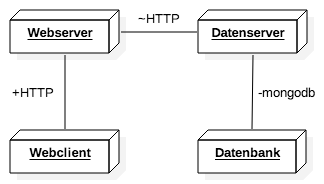
\includegraphics[width=14cm]{bilder/genereller_aufbau}
	\caption{Genereller Aufbau der Anwendung}
	\label{fig_genereller_aufbau}
\end{figure}

Wie in der Grafik zu sehen ist, besteht die Anwendung aus vier den Komponenten
\begin{itemize}
	\item \textbf{Webclient}: diese Komponente ist für den Nutzer sichtbar und dient der Interaktion mit der Anwendung
	\item \textbf{Webserver}: der Webserver nimmt Anfragen des Clients entgegen, beantwortet sie entweder selber oder leitet sie an den Datenserver weiter und gibt Antworten des Datenservers an den Webclient weiter
	\item \textbf{Datenserver}: der Datenserver nimmt Anfragen des Webservers entgegen und dient der Interaktion mit der Datenbank
	\item \textbf{Datenbank}: die Datenbank dient der persistenten Haltung von Sitzungsdaten und Fotos
\end{itemize}

Im Folgenden werden die einzelnen Komponenten im Detail vorgestellt und ihre Funktionsweise erläutert.